\documentclass{softengineering-lectures}
\graphicspath{{4_specifications/}}

\title{Спецификации программного обеспечения}

\author{Лекция №\,4 по курсу \newline <<Основы инженерии программого обеспечения>>}

\date{\small \copyright\ 2008--2009, 2012, 2016 Парамонов Илья Вячеславович}

\begin{document}

\begin{frame}
  \titlepage
\end{frame}

\begin{frame}{План лекции}
  \tableofcontents
\end{frame}

\section{Классификация и качества спецификаций}

\subsection{}

\begin{frame} \frametitle{Виды спецификаций}

  \begin{definition}
    \alert{Спецификация} "--- это документ, описывающий соглашения между двумя
    субъектами процесса разработки ПО и/или его эксплуатации
  \end{definition}
  
  \begin{itemize}
  \item Спецификация требований "--- соглашение между конечным
    пользователем и разработчиком системы
  \item Спецификация проекта "--- соглашение между архитектором системы и её
    конструкторами
  \item Спецификация модуля "--- соглашение между программистами реализующими и
    использующими данный модуль
  \end{itemize}
  
\end{frame}

\begin{frame} \frametitle{Цели написания спецификаций}

  \begin{itemize}
  \item Формулировка пользовательских требований
  \item Определение интерфейса между компьютером и~управляемой средой
  \item Формулировка требований к реализации
  \item Определение интерфейса между составляющими реализации
  \item Определение контрольных точек процесса разработки и~сопровождения ПО
  \item Определение правил эксплуатации продукта
  \end{itemize}
  
\end{frame}

\begin{frame} \frametitle{Качества спецификаций: чёткость, однозначность,
    понятность}

  \begin{definition}
    \alert{ Чёткость, однозначность, понятность} "--- это качества,
    гарантирующие правильное понимание требований спецификации и отсутствие
    возможных разночтений в этом понимании
  \end{definition}
  
  \begin{itemize}
  \item Необходимо создать три копии сообщения, которые должны отправляться по
    трём различным физическим каналам. Сообщение принимается адресатом с
    использованием голосования <<два из трёх>>
  \item \alert{ Должен ли адресат дожидаться третьей копии сообщения, если он
      уже получил две одинаковые? }
  \end{itemize}
  
\end{frame} 

\begin{frame} \frametitle{Качества спецификаций: согласованность}

  \begin{definition}
    \alert{Согласованность} означает отсутствие в спецификации противоречивых
    требований (удовлетворить таким требованиям не сможет никакая реализация)
  \end{definition}
  
  \begin{itemize}
  \item Никакая строка текста в текстовом редакторе не должна выходить за
    пределы заданной пользователем области текста
  \item При выключенном режиме расстановки переносов перенос осуществляется
    только по целым словам
  \item \alert{ Что делать, если режим расстановки переносов выключен и
      встретилось слово более длинное, чем установленная длина строки? }
  \end{itemize}    

\end{frame}

\begin{frame} \frametitle{Качества спецификаций: полнота}

  \begin{itemize}
  \item \alert{Внутренняя полнота} означает, что все используемые термины,
    понятия и концепции определены внутри самой спецификации
    \begin{itemize}
    \item При отсутствии невыполненных вызовов лифт должен находится в \alert{состоянии
      <<ожидания вызова>>}
    \end{itemize}
  \item \alert{Внешняя полнота} означает, что спецификация описывает все
    \alert{требуемые} характеристики системы
    \begin{itemize}
    \item После выполнения всех вызовов лифт должен возвращаться на первый этаж
    \item Объект, указатель на который передаётся методу \texttt{DoSomething()},
      будет удалён деструктором класса
    \end{itemize}
    Внешняя полнота часто недостижима, так как некоторые требования могут быть
    сформулированы только в~процессе эксплуатации системы
  \end{itemize}
  
\end{frame}

\begin{frame} \frametitle{Операционные и описательные спецификации}

  \begin{itemize}
  \item \alert{Описательная спецификация} "--- это спецификация, характеризующая
    \alert{желательные свойства} системы чисто декларативно
    \begin{itemize}
    \item Описательные спецификации, вообще говоря, не предполагают никакой явной
      схемы реализации
    \end{itemize}
  \item \alert{Операционная спецификация} "--- это спецификация, характеризующая
    систему через описание её \alert{желательного поведения}
    \begin{itemize}
    \item Операционные спецификации обычно предполагают способ
      реализации. Однако, реализация \alert{не обязана использовать именно этот
        способ}, достаточно лишь, чтобы система \alert{снаружи могла быть интерпретирована}
      способом, указанным в спецификации
    \end{itemize}
  \item Возможны также спецификации смешанного стиля
  \end{itemize}
  
\end{frame}

\begin{frame} \frametitle{Операционные и описательные спецификации: пример}

  Спецификация процедуры сортировки исходного списка \texttt{a}
  
  \begin{itemize}
  \item \alert{Описательная спецификация.} Результат сортировки "--- список
    \texttt{b}, являющийся упорядоченной перестановкой списка \texttt{a}
  \item \alert{Операционная спецификация.} Результат сортировки "--- список
    \texttt{b}, получаемый из списка \texttt{a} следующим образом:
    \begin{enumerate}
    \item Создать пустой список \texttt{b}
    \item Выбрать минимальный элемент списка \texttt{a} и перенести его в~конец
      списка \texttt{b}
    \item Повторять предыдущий шаг пока список \texttt{a} не станет пустым
    \end{enumerate}
  \item \alert{Смешанная спецификация} сортировки с удалением дубликатов:
    \begin{enumerate}
    \item Построить список \texttt{b}, являющийся упорядоченной перестановкой списка
      \texttt{a}
    \item Удалить все дублирующиеся элементы из списка \texttt{b}
    \end{enumerate}    
  \end{itemize}
  
\end{frame}

%\section{Описательные спецификации}

\section{Способы представления операционных и~описательных спецификаций}

\subsection{}

\begin{frame}
  \frametitle{Спецификации сценариев использования}

  \begin{itemize}
  \item \alert{Сценарий использования (use case)} "--- это описание типичного
    способа взаимодействия пользователя с~системой и её функционирования в ходе
    данного взаимодействия
  \item \alert{Актёр (actor)} "--- участник системы, предпринимающий по
    отношению к ней какие-либо активные действия, движимый некоторой конкретной
    целью. Термин является неудачным, точнее было бы использовать слово
    \alert{роль}
  \end{itemize}

  Основное назначение сценариев использования "--- передавать информацию о
  предполагаемых способах использования системы от заказчика к разработчику
\end{frame}

\begin{frame}
  \frametitle{Диаграмма сценариев использования}

  \centerline{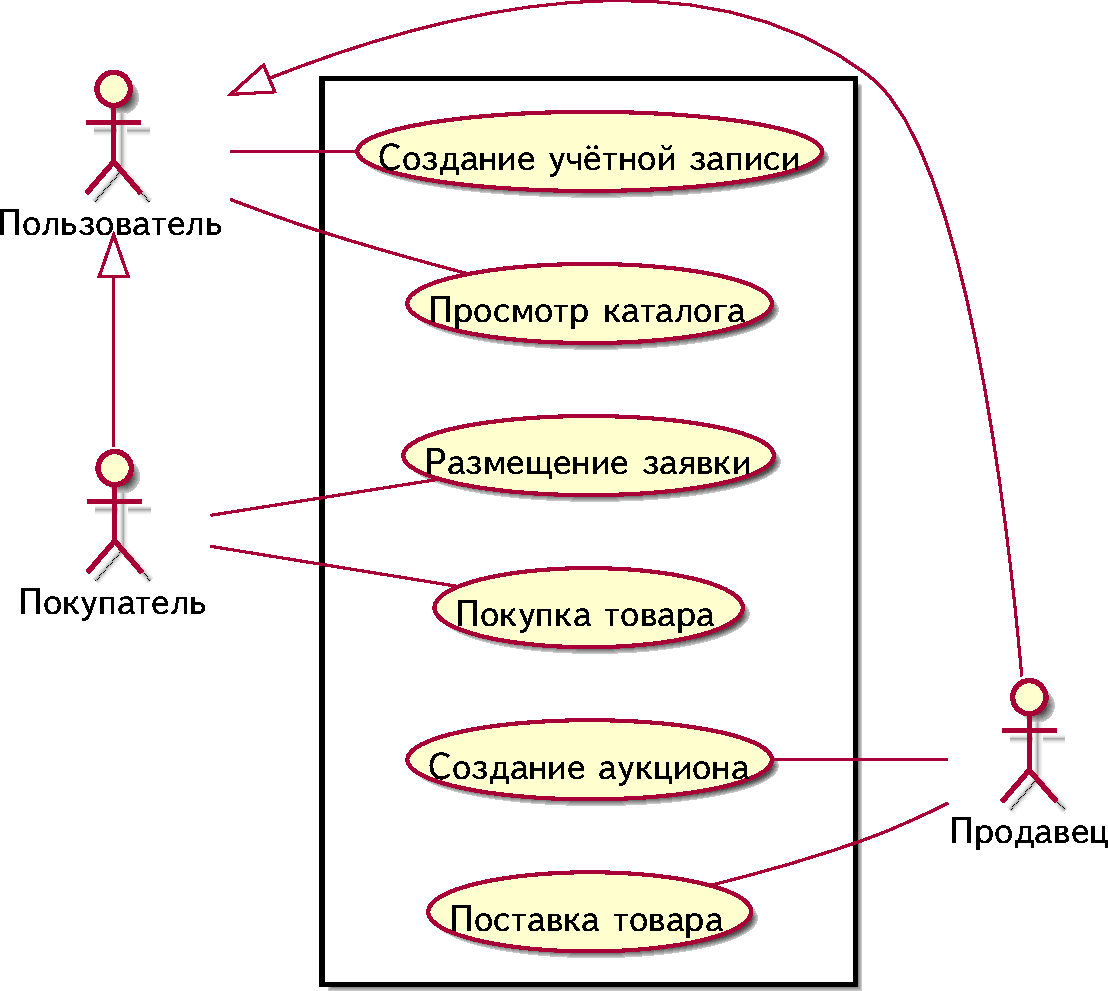
\includegraphics[height=0.9\textheight]{usecase.pdf}}
\end{frame}

\begin{frame}
  \frametitle{Пример сценария использования (начало)}

  \begin{tabular}{|l|l|}
    \hline
    Use case No. & 14 \\
    Application & Интернет-магазин \\
    Use case name & Покупка товара \\
    Primary actor & Покупатель \\
    Use case description & Пользователь выбирает товары из каталога \\
    & с целью их покупки, оплачивает покупку \\
    & и сообщает данные, необходимые для \\
    & доставки\\
    Precondition & система не находится в режиме\\
    & технического обслуживания \\
    Trigger & нет\\
    \hline
  \end{tabular}
\end{frame}

\begin{frame}
  \frametitle{Пример сценария использования (продолжение)}

  \textbf{Basic flow}
  \begin{enumerate}
  \item[1] Покупатель просматривает каталог и выбирает товары для покупки
  \item[2] Покупатель оценивает стоимость всех товаров
  \item[3] Покупатель вводит информацию, необходимую для доставки
  \item[4] Система предоставляет полную информацию о цене товара и его доставке
  \item[5] Покупатель вводит данные кредитной карточки
  \item[6] Система осуществляет авторизацию счёта покупателя
  \item[7] Система подтверждает оплату товара
  \item[8] Система посылает подтверждение оплаты товара по e-mail
  \end{enumerate}
\end{frame}

\begin{frame}
  \frametitle{Пример сценария использования (окончание)}

  \textbf{Alternate flows}
  \begin{enumerate}
  \item[3a] Покупатель является постоянным клиентом
  \item[.1] Система предоставляет полную информацию о товаре и состоянии счёта заказчика
  \item[.2] Покупатель может согласиться или изменить значения по умолчанию,
    после чего осуществляется переход к шагу \textcolor{blue}{6}
  \item[6a] Система не подтверждает авторизацию счёта
  \item[.1] Покупатель может повторить ввод информации кредитной карты или
    отказаться от покупки
  \end{enumerate}
\end{frame}

\begin{frame} \frametitle{Спецификации предметной области}

  \begin{itemize}
  \item ER-диаграммы
    \begin{itemize}
    \item Представляют собой первое приближение к описанию структуры предметной
      области, базы данных и/или структуры классов
    \item Может рассматриваться на различных уровнях (только сущности и связи;
      модели, основанные на ключах; полные атрибутивные модели)
    \item Могут быть понятны как разработчику, так и заказчику
    \end{itemize}
  \item Диаграммы классов
    \begin{itemize}
    \item Основной инструмент спецификации при проектировании
    \item В требуемой степени детальности показывают структурные аспекты
      системы, а также её потенциальные возможности
    \item Не определяют реального механизма взаимодействия компонентов
      и~выполнения операций
    \end{itemize}
  \item Текстовые спецификации
  \end{itemize}
  
\end{frame}

\begin{frame} \frametitle{Диаграммы потоков данных (DFD)}

  \centerline{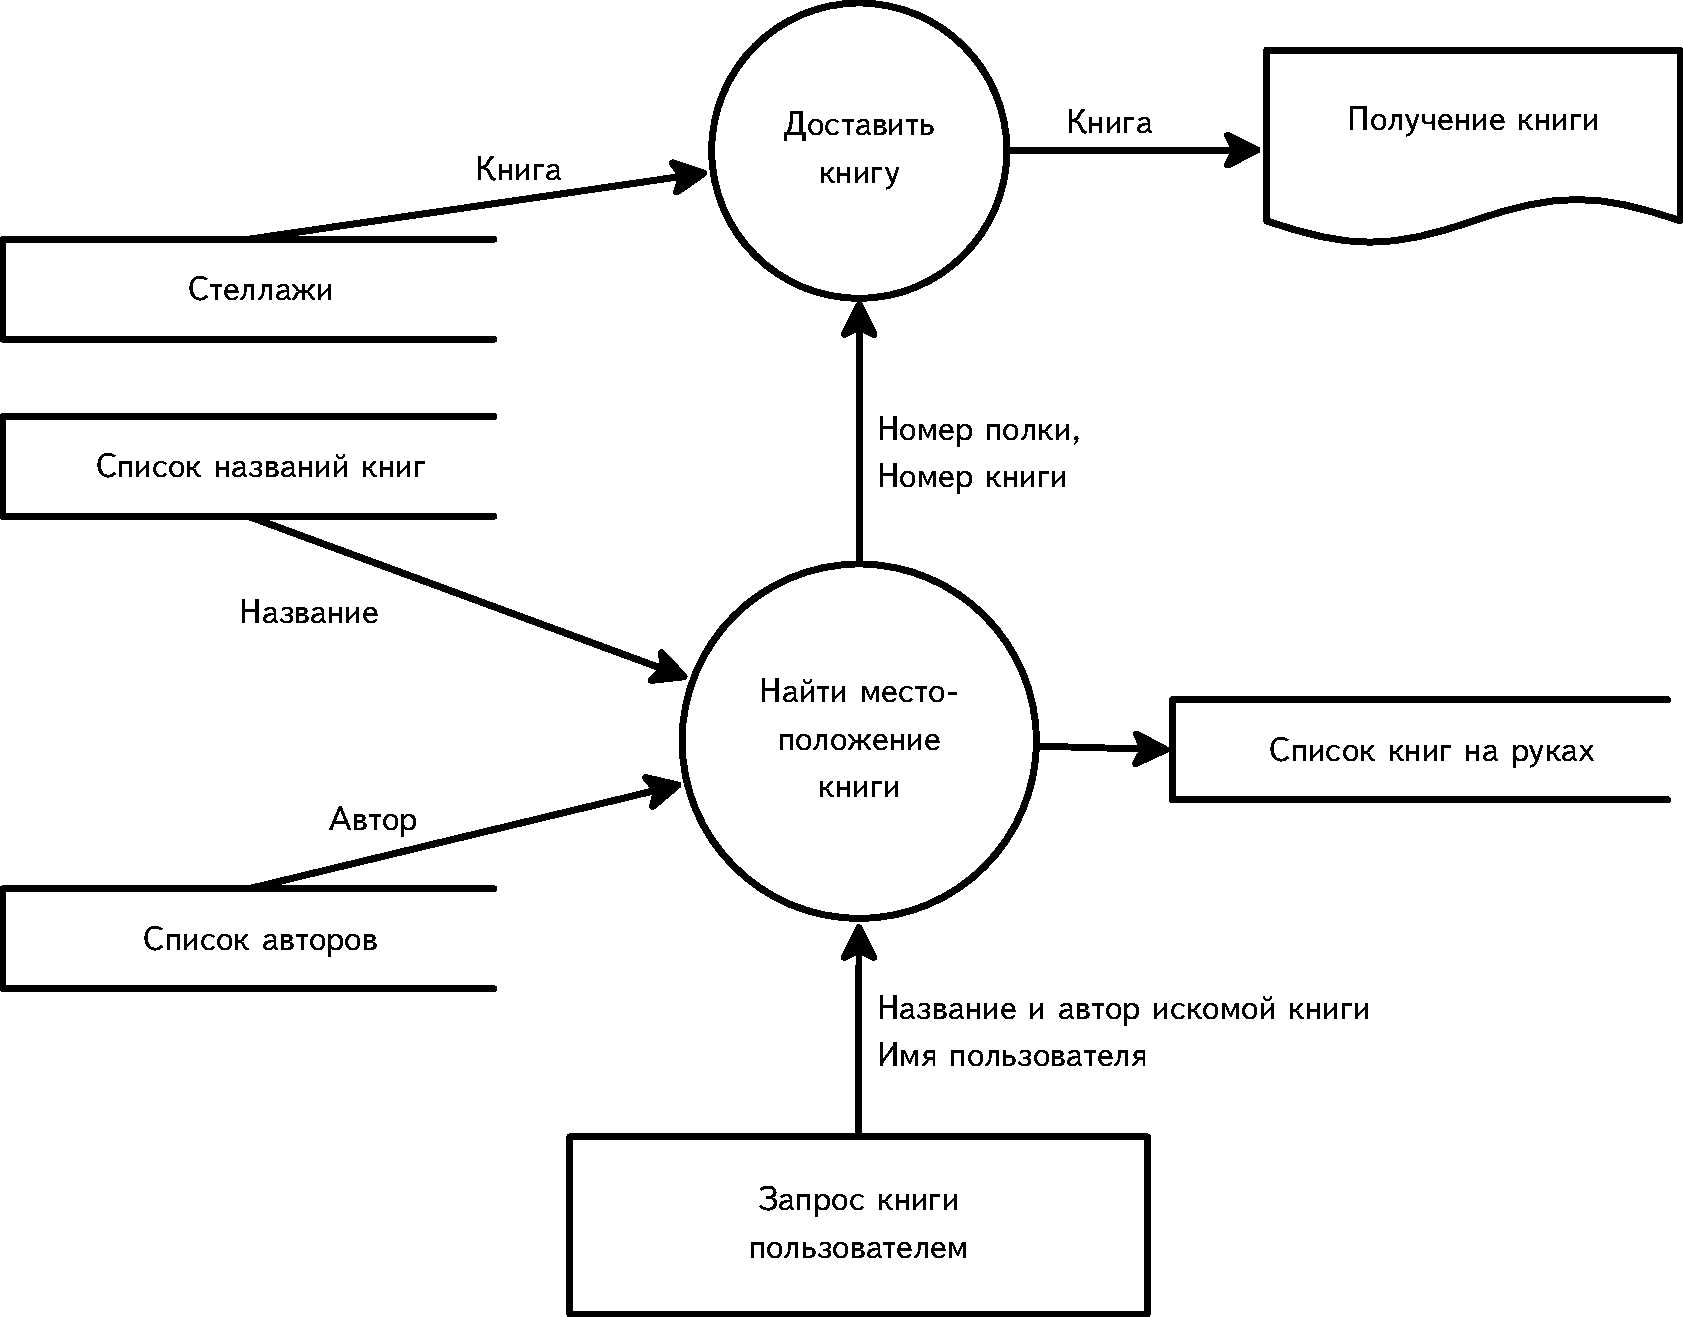
\includegraphics[width=0.9\textwidth]{dfd.pdf}}

\end{frame}

\begin{frame} \frametitle{Диаграммы состояний (UML)}

  \centerline{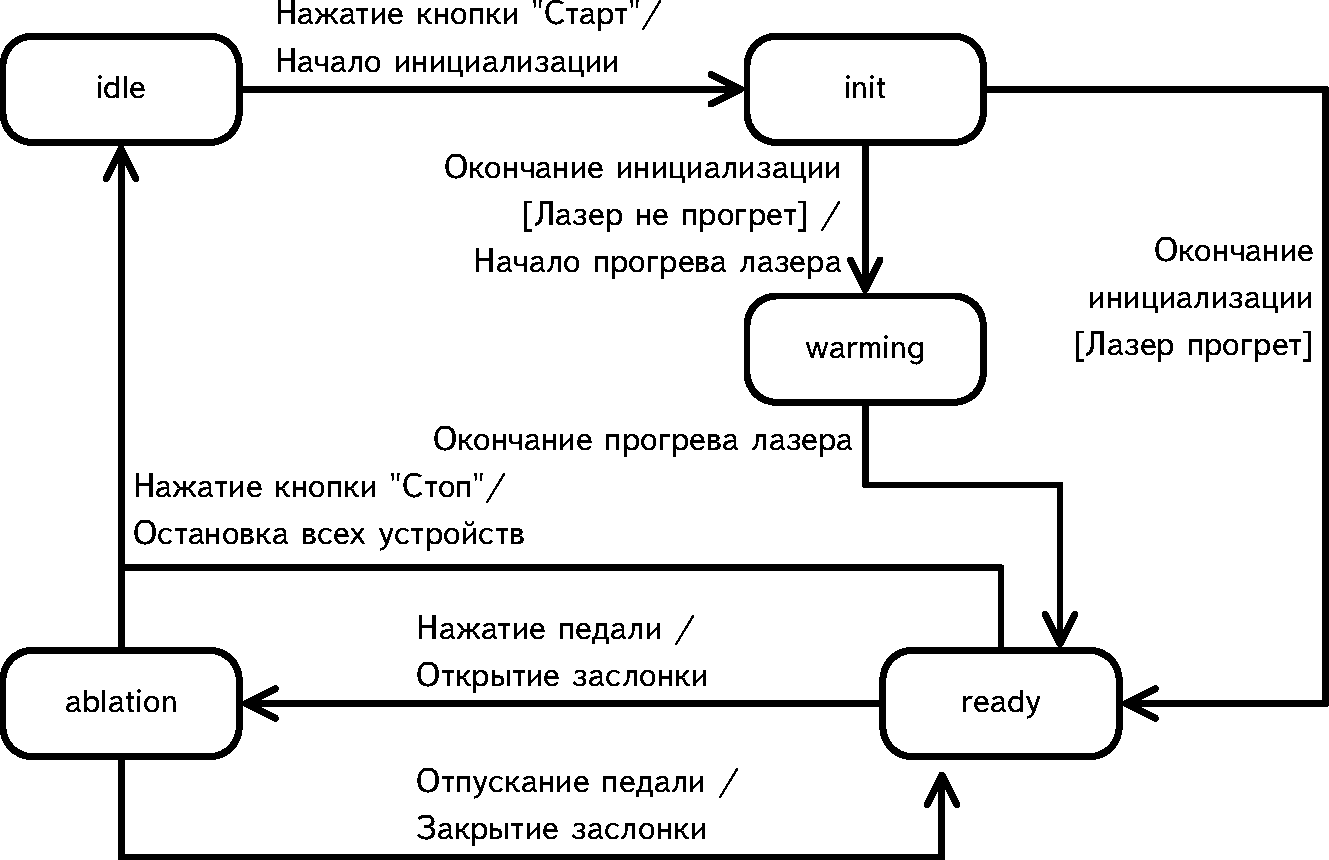
\includegraphics[width=0.9\textwidth]{states1.pdf}}

\end{frame}

\begin{frame} \frametitle{Реализация диаграмм состояний}
  \begin{itemize}
  \item Вложенный оператор \texttt{switch}
    \begin{itemize}
    \item Самая простая реализация
    \item Плохо масштабируется, код становится громоздким и трудночитаемым уже
      для диаграмм среднего размера
    \end{itemize}
  \item Таблица переходов
    \begin{itemize}
    \item Требуемая инфраструктура реализуется один раз
    \item Таблица переходов может быть изменена без перекомпиляции
    \item Несколько ограниченные возможности реализации кода
    \end{itemize}
  \item Шаблон проектирования \emph{State}
    \begin{itemize}
    \item Решение является объектно"=ориентированным
    \item Хорошо масштабируется, код обработки каждого состояния локализован
      в~одном классе
    \item Может быть несколько громоздким в простых случаях
    \end{itemize}
  \end{itemize}
\end{frame}

\begin{frame} \frametitle{Диаграммы последовательности (UML)}

    \centerline{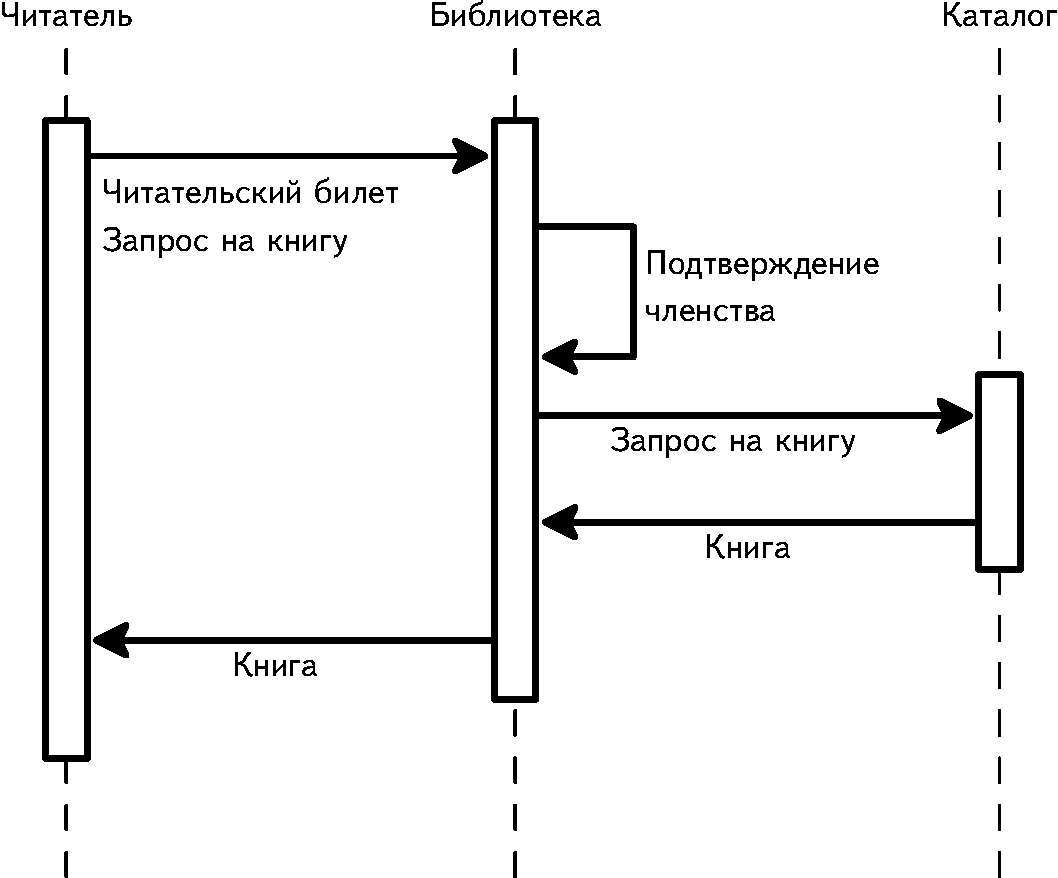
\includegraphics[height=0.8\textheight]{sequence.pdf}}

\end{frame}

\begin{frame} \frametitle{Диаграммы деятельности (UML)}

  \centerline{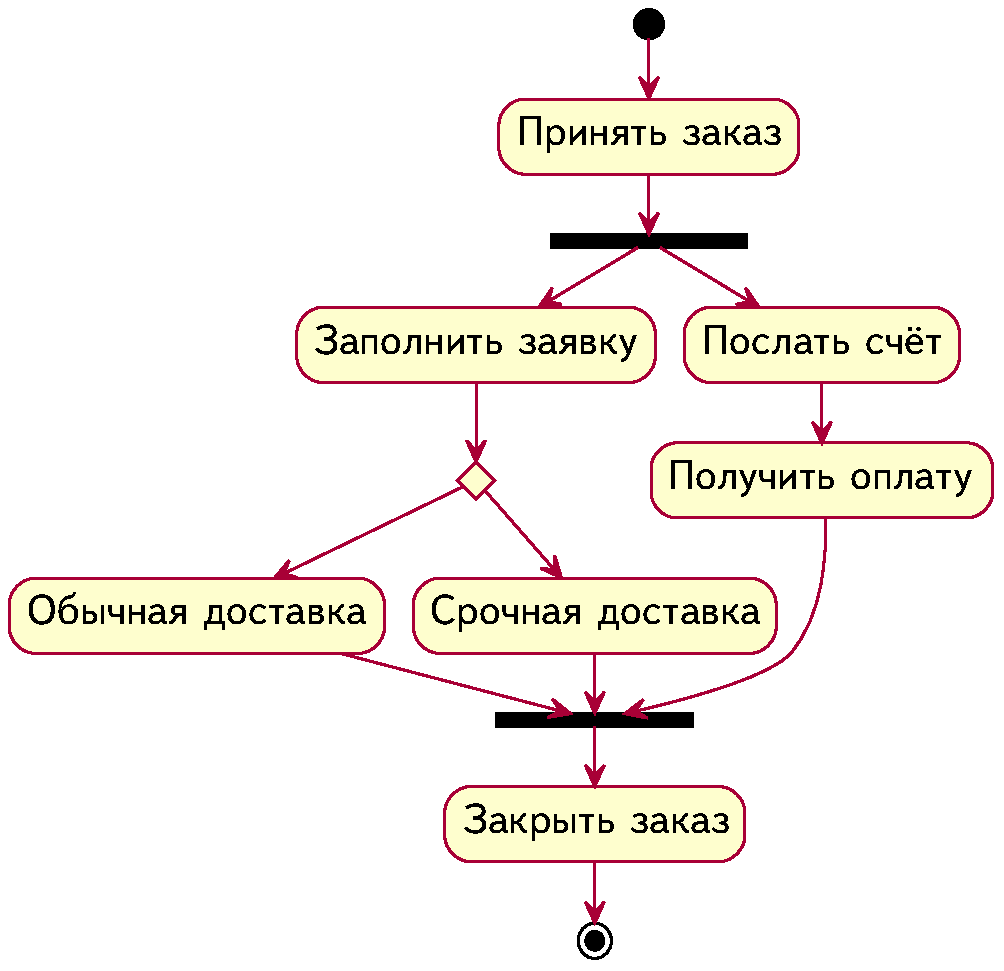
\includegraphics[height=0.9\textheight]{activity.pdf}}

\end{frame}

\begin{frame} \frametitle{Модульные спецификации}
  \begin{itemize}
  \item Документация верхнего уровня: Start Here (корневые объекты)
  \item Документация классов: назначение, интерфейсы, способ создания объектов,
    пример использования
  \item Документация методов:
    \begin{itemize}
    \item входные условия, выходные условия и инварианты
    \item как метод воздействует на состояние объекта\\ (без деталей реализации!)
    \item коды возврата и выбрасываемые исключения
    \item побочные эффекты
    \item зависимые виртуальные методы
    \item поточная безопасность
    \end{itemize}
  \end{itemize}
\end{frame}

\section{}

\begin{frame} \frametitle{Вопросы к~семинару}
  \small
  \begin{enumerate}
  \item Определите, какие качества ПО пригодны для специфицирования, и каким
    образом могут выглядеть соответствующие спецификации
  \item Обсудите применение к пострению спецификаций принципов общности и
    предусмотрения изменений
  % \item Постройте диаграмму DFD, описывающую операции добавления, изменения и
  %   удаления информации о сотрудниках некоторой организации, а также операцию
  %   вычисления зарплаты сотрудников на основе базовой ставки и фактически
  %   отработанного времени
  \item Опишите процедуру преобразования диаграммы состояний в~код в
    соответствии c шаблоном проектирования \emph{State}
  \item Предложите механизм трансляции диаграмм деятельности на языке UML в
    программный код на языке Java (с~использованием средств многопоточности последнего)
  \end{enumerate}
  \alert{Стремитесь быть конкретными в~ответах! Приводите примеры!}
\end{frame}

\begin{frame} \frametitle{Задание к семинару}
  \begin{itemize}
  \item Система состоит из нескольких лифтов, перемещающихся между этажами
  \item В каждой лифтовой кабине имеется набор кнопок, по одной для каждого
    этажа. При нажатии кнопки загораются и кабина перемещается на указанный
    этаж. По достижении нужного этажа кнопка гаснет
  \item Каждый этаж (кроме первого и последнего) имеет две кнопки: вызов лифта
    для движения вверх и вниз. При нажатии эти кнопки загораются. Кнопки гаснут,
    когда лифт достигает указанного этажа и затем либо перемещается в нужном
    направлении, либо не имеет невыполненных вызовов. Если были нажаты обе
    кнопки вызова на этаж, то гаснет только одна
  \end{itemize}
  Специфицируйте такую систему лифтов
\end{frame}

\end{document}

%%% Local Variables: 
%%% mode: TeX-pdf
%%% TeX-master: t
%%% End: 
